% Created 2014-03-28 Fri 08:57
\documentclass[table,smaller]{beamer}
\usepackage[utf8]{inputenc}
\usepackage[T1]{fontenc}
\usepackage{fixltx2e}
\usepackage{graphicx}
\usepackage{longtable}
\usepackage{float}
\usepackage{wrapfig}
\usepackage{rotating}
\usepackage[normalem]{ulem}
\usepackage{amsmath}
\usepackage{textcomp}
\usepackage{marvosym}
\usepackage{wasysym}
\usepackage{amssymb}
\usepackage{hyperref}
\tolerance=1000
\usepackage{tikz}
\usepackage{minted}
\usepackage{fancyvrb}
\usemintedstyle{perldoc}
\definecolor{lightgray}{gray}{0.96}
\setlength{\tabcolsep}{1ex}
\institute{Harvard MIT Data Center}
\usetheme{Warsaw}
\useoutertheme{infolines}
\setbeamercolor{block body}{bg=lightgray}
\titlegraphic{
\includegraphics[width=.75\textwidth]{images/IQSSNewLogo.pdf}}
\setbeamersize{text margin left=2em,text margin right=2em}
\AtBeginSection[]{\begin{frame}<beamer>\frametitle{Topic}\tableofcontents[currentsection]\end{frame}}
\usetheme{default}
\author{}
\date{}
\title{Data Management in Stata}
\hypersetup{
  pdfkeywords={},
  pdfsubject={},
  pdfcreator={Emacs 24.3.1 (Org mode 8.2.5h)}}
\begin{document}

\maketitle
\begin{frame}{Outline}
\tableofcontents
\end{frame}


\section{Introduction}
\label{sec-1}
\rowcolors{1}{blue!15}{blue!3}
\definecolor{bg}{rgb}{0.95,0.95,0.95}
\definecolor{cbg}{cmyk}{0,0,.1,0}

\begin{frame}[fragile,label=sec-1-1]{Materials and Setup}
 \begin{itemize}
\item Lab computer log in:
\begin{itemize}
\item USERNAME: dataclass
\item PASSWORD: dataclass
\end{itemize}
\item Workshop materials:
\begin{itemize}
\item Download class materials from \url{http://j.mp/stata-datman}
\item Open a file browser, right-click on \texttt{StataDatMan.zip}, select the \texttt{WinZip} menu and select \texttt{Extrat to Here}.
\end{itemize}
\end{itemize}
\end{frame}
\begin{frame}[label=sec-1-2]{Workshop Description}
\begin{itemize}
\item This is an Introduction to data management in Stata
\item Assumes basic knowledge of Stata
\item Not appropriate for people already well familiar with Stata
\item If you are catching on before the rest of the class, experiment with command features described in help files
\end{itemize}
\end{frame}
\begin{frame}[label=sec-1-3]{Organization}
\begin{itemize}
\item Please feel free to ask questions at any point if they are relevant to the current topic (or if you are lost!)
\item There will be a Q\&A after class for more specific, personalized questions
\item Collaboration with your neighbors is encouraged
\item If you are using a laptop, you will need to adjust paths accordingly
\end{itemize}
\end{frame}
\begin{frame}[fragile,label=sec-1-4]{Opening Files in Stata}
 \begin{itemize}
\item Look at bottom left hand corner of Stata screen
\begin{itemize}
\item This is the directory Stata is currently reading from
\end{itemize}
\item Files are located in the StataDatMan folder in your home directory
\item Start by telling Stata where to look for these
\end{itemize}
\vspace{-.5em} \begin{columns} \column{.85\linewidth} \begin{block}{}
\begin{minted}[fontsize=\footnotesize]{c}
// change directory
cd "C:/Users/dataclass/Desktop/StataDatMan"

// Use dir to see what is in the directory:
dir
dir dataSets

// use the gss data set
use dataSets/gss.dta
\end{minted}
\end{block} \end{columns}
\end{frame}
\section{Generating and replacing variables}
\label{sec-2}

\begin{frame}[label=sec-2-1]{Basic Data Manipulation Commands}
Basic commands you'll use for generating new variables or recoding existing variables:
\begin{itemize}
\item gen
\item egen
\item replace
\item recode
\end{itemize}
Many different means of accomplishing the same thing in Stata -- find what is comfortable (and easy) for you!
\end{frame}
\begin{frame}[fragile,label=sec-2-2]{Generate and Replace}
 The \verb~replace~ command is often used with logic statements. Available logical operators include the following:
\begin{description}
\item[{==}] equal to (status quo)
\item[{!=}] not equal to
\item[{>}] greater than
\item[{<}] less than
\item[{>=}] greater than or equal to
\item[{<=}] less than or equal to
\item[{\&}] and
\item[{|}] or
\end{description}

For example:

\vspace{-.5em} \begin{columns} \column{.85\linewidth} \begin{block}{}
\begin{minted}[fontsize=\footnotesize]{c}
// create "hapnew" variable
gen hapnew = . //set to missing
//set to 0 if happy equals 1
replace hapnew=0 if happy==1 
//set to 1 if happy both and hapmar are greater than 3
replace hapnew=1 if happy>3 & hapmar>3
tab hapnew // tabulate the new variable
\end{minted}
\end{block} \end{columns}
\end{frame}
\begin{frame}[fragile,label=sec-2-3]{Recode}
 The \verb~recode~ command is basically generate and replace combined. You can recode an existing variable OR use recode to create a new variable (via the \verb~gen~ option).

\vspace{-.5em} \begin{columns} \column{.85\linewidth} \begin{block}{}
\begin{minted}[fontsize=\footnotesize]{c}
// recode the wrkstat variable 
recode wrkstat (1=8) (2=7) (3=6) (4=5) (5=4) (6=3) (7=2) (8=1)
// recode wrkstat into a new variable named wrkstat2
recode wrkstat (1=8), gen(wrkstat2)
// tabulate workstat
tab wrkstat
\end{minted}
\end{block} \end{columns}

\begin{itemize}
\item The table below illustrates common forms of recoding
\end{itemize}
\begin{center}
\begin{tabular}{lll}
Rule & Example & Meaning\\
\hline
\#=\# & 3=1 & 3 recoded to 1\\
\#\#=\# & 2. =9 & 2 and . recoded to 9\\
\#/\# = \# & 1/5=4 & 1 through 5 recoded to 4\\
nonmissing=\# & nonmiss=8 & nonmissing recoded to 8\\
missing=\# & miss=9 & missing recoded to 9\\
\end{tabular}
\end{center}
\end{frame}

\begin{frame}[fragile,label=sec-2-4]{egen}
 The \verb~egen~ command ("extensions" to the \verb~gen~ command) provides convenient methods for performing many common data manipulation tasks.

For example, we can use \verb~egen~ to create a new variable that counts the number of "yes" responses on computer, email and internet use:
\vspace{-.5em} \begin{columns} \column{.85\linewidth} \begin{block}{}
\begin{minted}[fontsize=\footnotesize]{c}
// count number of yes on use comp email and net 
egen compuser= anycount(usecomp usemail usenet), values(1)
tab compuser
\end{minted}
\end{block} \end{columns}

Here are some additional examples of \verb~egen~ in action:
\vspace{-.5em} \begin{columns} \column{.85\linewidth} \begin{block}{}
\begin{minted}[fontsize=\footnotesize]{c}
// assess how much missing data each participant has:
egen countmiss = rowmiss(age-wifeft)
codebook countmiss
// compare values on multiple variables
egen ftdiff=diff(wkftwife wkfthusb)
codebook ftdiff
\end{minted}
\end{block} \end{columns}


You will need to refer to the documentation to discover what else \verb~egen~ can do: type "help egen" in Stata to get a complete list of functions.
\end{frame}
\begin{frame}[label=sec-2-5]{Exercise 1: Generate, Replace, Recode \& Egen}
Open the gss.dta data.
\begin{enumerate}
\item Generate a new variable that represents the squared value of age.
\item Generate a new variable equal to "1" if income is greater than "19".
\item Create a new variable that counts the number of missing responses for each respondent.
\end{enumerate}
\end{frame}

\section{By processing}
\label{sec-3}

\begin{frame}[fragile,label=sec-3-1]{The "bysort" Command}
 Sometimes, you'd like to create variables based on different categories of a single variable. For example, say you want to look at happiness based on whether an individual is male or female. The "bysort" prefix does just this:

\vspace{-.5em} \begin{columns} \column{.85\linewidth} \begin{block}{}
\begin{minted}[fontsize=\footnotesize]{c}
// tabulate happy separately for male and female 
bysort sex: tab happy
// generate summary statistics using bysort 
bysort state: egen stateincome = mean(income)
bysort degree: egen degreeincome = mean(income)
bysort marital: egen marincomesd = sd(income)
\end{minted}
\end{block} \end{columns}
\end{frame}
\begin{frame}[fragile,label=sec-3-2]{By prefix vs. by options}
 Some commands won't work with by prefix, but instead have a \verb~by~ option:

\vspace{-.5em} \begin{columns} \column{.85\linewidth} \begin{block}{}
\begin{minted}[fontsize=\footnotesize]{c}
// generate separate histograms for female and male 
hist nethrs, by(sex)
\end{minted}
\end{block} \end{columns}

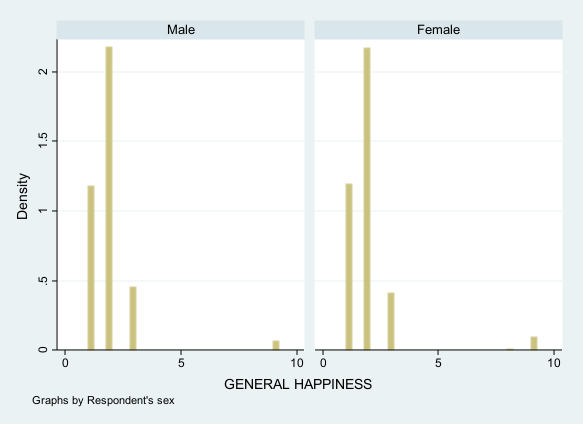
\includegraphics[width=.9\linewidth]{images/histBysex.png}
\end{frame}

\section{Missing values}
\label{sec-4}

\begin{frame}[fragile,label=sec-4-1]{Missing Values}
 You always need to consider how missing values are coded when recoding variables.

\begin{itemize}
\item Stata's symbol for a missing value is "."
\item Stata interprets "." as a large value
\item Easy to make mistakes!
\end{itemize}
To identify highly educated women, we might use the command:

\vspace{-.5em} \begin{columns} \column{.85\linewidth} \begin{block}{}
\begin{minted}[fontsize=\footnotesize]{c}
// generate and replace without considering missing values
gen hi_ed=0
replace hi_ed=1 if wifeduc>15
// What happens to our missing values?
tab hi_ed, mi nola
\end{minted}
\end{block} \end{columns}

It looks like around 66\% have higher education, but look closer:

\vspace{-.5em} \begin{columns} \column{.85\linewidth} \begin{block}{}
\begin{minted}[fontsize=\footnotesize]{c}
// gen hi_ed2, but don't set a value if wifeduc is missing
gen hi_ed2 = 0 if wifeduc != . 
// only replace non-missing
replace hi_ed2=1 if wifeduc >15 & wifeduc !=. 
tab hi_ed2, mi //check to see that missingness is preserved
\end{minted}
\end{block} \end{columns}

The correct value is 10\%. Moral of the story? Be careful with missing values and remember that Stata considers missing values to be large!
\end{frame}
\begin{frame}[fragile,label=sec-4-2]{Bulk Conversion to Missing Values}
 Often the data collection/generating procedure will have used some other value besides "." to represent missing values. The \verb~mvdecode~ command will convert all these values to missing. For example:

\vspace{-.5em} \begin{columns} \column{.85\linewidth} \begin{block}{}
\begin{minted}[fontsize=\footnotesize]{c}
mvdecode _all, mv(999)
\end{minted}
\end{block} \end{columns}

\begin{itemize}
\item The "$\backslash$$_{\text{all}}$" command tells Stata to do this to all variables
\item Use this command carefully!
\begin{itemize}
\item If you have any variables where "999" is a legitimate value,
Stata is going to recode it to missing
\item As an alternative, you could list var names separately rather
than using "$\backslash$$_{\text{all}}$"
\end{itemize}
\end{itemize}
\end{frame}
\section{Variable types}
\label{sec-5}

\begin{frame}[label=sec-5-1]{Variable Types}
Stata uses two main types of variables: String and Numeric. To be able to perform any mathematical operations, your variables need to be in a numeric format. Stata can store numbers with differing levels of precision, as described in the table below.

\begin{center}
\begin{tabular}{llllr}
type & Minimum & Maximum & being 0 & bytes\\
\hline
byte & -127 & 100 & +/-1 & 1\\
int & -32,767 & 32,740 & +/-1 & 2\\
long & -2,147,483,647 & 2,147,483,620 & +/-1 & 4\\
float & -1.70141173319*10$^{\text{38}}$ & 1.70141173319*10$^{\text{38}}$ & +/-10$^{\text{-38}}$ & 4\\
double & -8.9884656743*10$^{\text{307}}$ & 8.9884656743*10$^{\text{307}}$ & +/-10$^{\text{-323}}$ & 8\\
\end{tabular}
\end{center}
\begin{itemize}
\item Precision for float is 3.795x10$^{\text{-8}}$.
\item Precision for double is 1.414x10$^{\text{-16}}$.
\end{itemize}
\end{frame}
\begin{frame}[fragile,label=sec-5-2]{Converting to and from Strings}
 Stata provides several ways to convert to and from strings. You can use \verb~tostring~ and \verb~destring~ to convert from one type to the other:

\vspace{-.5em} \begin{columns} \column{.85\linewidth} \begin{block}{}
\begin{minted}[fontsize=\footnotesize]{c}
// convert degree to a string
tostring degree, gen(degree_s)
// and back to a number
destring degree_s, gen(degree_n)
\end{minted}
\end{block} \end{columns}

Use \verb~decode~ and \verb~encode~ to convert to/from variable labels:

\vspace{-.5em} \begin{columns} \column{.85\linewidth} \begin{block}{}
\begin{minted}[fontsize=\footnotesize]{c}
// convert degree to a descriptive string
decode degree, gen(degree_s2)
// and back to a number with labels
encode degree_s2, gen(degree_n2)
\end{minted}
\end{block} \end{columns}
\end{frame}
\begin{frame}[fragile,label=sec-5-3]{Converting Strings to Date/Time}
 Often date/time variables start out as strings -- You'll need to convert them to numbers using one of the conversion functions listed below.

\begin{center}
\begin{tabular}{lll}
Format & Meaning & String-to-numeric conversion function\\
\hline
\%tc & milliseconds & clock(string, mask)\\
\%td & days & date(string, mask)\\
\%tw & weeks & weekly(string, mask)\\
\%tm & months & monthly(string, mask)\\
\%tq & quarters & quarterly(string, mask)\\
\%ty & years & yearly(string, mask)\\
\hline
\end{tabular}
\end{center}

Date/time variables are stored as the number of units elapsed since 01jan1960 00:00:00.000. For example, the \verb~date~ function returns the number of days since that time, and the \verb~clock~ function returns the number of milliseconds since that time.

\vspace{-.5em} \begin{columns} \column{.85\linewidth} \begin{block}{}
\begin{minted}[fontsize=\footnotesize]{c}
// create string variable and convert to date
gen date = "November 9 2020"
gen date1 = date(date, "MDY")
list date1 in 1/5
\end{minted}
\end{block} \end{columns}
\end{frame}
\begin{frame}[fragile,label=sec-5-4]{Formatting Numbers as Dates}
 Once you have converted the string to a number you can format it for display. You can simply accept the defaults used by your formatting string or provide details to customize it.

\vspace{-.5em} \begin{columns} \column{.85\linewidth} \begin{block}{}
\begin{minted}[fontsize=\footnotesize]{c}
// format so humans can read the date
format date1 %d
list date1 in 1/5
// format with detail
format date1 %tdMonth_dd,_CCYY
list date1 in 1/5
\end{minted}
\end{block} \end{columns}
\end{frame}
\begin{frame}[label=sec-5-5]{Exercise 2: Missing Values, String Conversion, and by Processing}
\begin{enumerate}
\item Recode values "99" and "98" on the variable, "hrs1"  as "missing."
\item Recode the marital variable into a "string" variable and then back into a numeric variable.
\item Create a new variable that associates each individual with the average number of hours worked among individuals with matching educational degrees (see the last "by" example for inspiration).
\end{enumerate}
\end{frame}
\section{Merging, appending, and joining}
\label{sec-6}

\begin{frame}[fragile,label=sec-6-1]{Merging Datasets}
 You can \verb~merge~ variables from a second dataset to the dataset you're currently working with.
\begin{itemize}
\item Current active dataset = master dataset
\item Dataset you'd like to merge with master = using dataset
\end{itemize}

There are different ways that you might be interested in merging data:
\begin{itemize}
\item Two datasets with same participant pool, one row per participant (1:1)
\item A dataset with one participant per row with a dataset with multiple rows per participant (1:many or many:1)
\end{itemize}
\end{frame}
\begin{frame}[fragile,label=sec-6-2]{Merging Datasets}
 Before you begin:
\begin{itemize}
\item Identify the "ID" that you will use to merge your two datasets
\item Determine which variables you'd like to merge
\item In Stata >= 11, data does NOT have to be sorted
\item Variable types must match across datasets (there is a "force" option to get around this, but not recommended)
\end{itemize}

Example: Let's say that we had one dataset with individual students (master) and another  dataset with information about the students' schools called "school.dta". We would merge these as follows:

\vspace{-.5em} \begin{columns} \column{.85\linewidth} \begin{block}{}
\begin{minted}[fontsize=\footnotesize]{c}
// Not run: conceptual example only. Merge school and student data
merge m:1 schoolID using school.dta
\end{minted}
\end{block} \end{columns}
\end{frame}
\begin{frame}[label=sec-6-3]{Merge Options}
There are several options that provide more fine-grain control over how the merge is carried out:
\begin{itemize}
\item In standard merge, the master dataset is the authority and WON'T CHANGE
\item If your master dataset has missing data and some of those values are not missing in your using dataset, specify "update" -- this will fill in missing data in master
\item If you want data from your using dataset to overwrite that in your master, specify "replace update" -- this will replace master data with using data UNLESS the value is missing in the using dataset
\end{itemize}
\end{frame}

\begin{frame}[fragile,label=sec-6-4]{Appending Datasets}
 Sometimes you have observations in two  different datasets, or you'd like to add  observations to an existing dataset. In this case you can use the \verb~append~ command to add observations to the end of the observations in the master dataset. For example:

\vspace{-.5em} \begin{columns} \column{.85\linewidth} \begin{block}{}
\begin{minted}[fontsize=\footnotesize]{c}
// Not run: conceptual example. add rows of data from dataset2 
append using dataset2
\end{minted}
\end{block} \end{columns}

To keep track of where observations came from, use the \verb~generate~ option as shown below:

\vspace{-.5em} \begin{columns} \column{.85\linewidth} \begin{block}{}
\begin{minted}[fontsize=\footnotesize]{c}
// Not run: conceptual example.
append using dataset1, generate(observesource)
\end{minted}
\end{block} \end{columns}

There is a "force" option will allow for data type mismatches, but again this is not recommended.
\end{frame}
\section{Creating summarized data sets}
\label{sec-7}

\begin{frame}[fragile,label=sec-7-1]{Collapse}
 Collapse will take master data and create a new dataset of summary statistics
\begin{itemize}
\item Useful in hierarchical linear modeling if you'd like to create aggregate, summary statistics
\item Can generate group summary data for many  descriptive stats
\item Can also attach weights
\end{itemize}

Before you collapse:
\begin{itemize}
\item Save your master dataset and then save it again under a new name (this will prevent collapse from writing over your original data\_
\item Consider issues of missing data. Do you want Stata to use all possible observations? If not, the \verb~cw~ (casewise) option will make casewise deletions
\end{itemize}
\end{frame}
\begin{frame}[fragile,label=sec-7-2]{Collapse Example}
 Suppose you have a dataset with patient  information from multiple hospitals and you want to generate mean levels of patient satisfaction for hospital: 

\vspace{-.5em} \begin{columns} \column{.85\linewidth} \begin{block}{}
\begin{minted}[fontsize=\footnotesize]{c}
// Not run: conceptual example. calculate average ptsatisfaction by hospital
save originaldata
collapse (mean) ptsatisfaction, by(hospital)
save hospitalcollapse
\end{minted}
\end{block} \end{columns}

You could also generate different statistics for multiple variables

\vspace{-.5em} \begin{columns} \column{.85\linewidth} \begin{block}{}
\begin{minted}[fontsize=\footnotesize]{c}
// create mean ptsatisfaction, median ptincome, sd ptsatisfaction for each hospital
collapse (mean) ptsatisfaction (median) ptincome (sd) ptsatisfaction, by(hosptial)
\end{minted}
\end{block} \end{columns}
\begin{itemize}
\item What if you want to rename your new variables in
this process?
\end{itemize}

\vspace{-.5em} \begin{columns} \column{.85\linewidth} \begin{block}{}
\begin{minted}[fontsize=\footnotesize]{c}
// Same as previous example, but rename variables
collapse (mean) ptsatmean=ptsatisfaction (median) ptincmed=ptincome
 (sd) sdptsat=ptsatisfaction, by(hospital)
\end{minted}
\end{block} \end{columns}
\end{frame}
\begin{frame}[label=sec-7-3]{Exercise 3: Merge, Append, and Collapse}
Open the gss2.dta dataset. This dataset contains only half of the variables that are in the complete gss dataset. 
\begin{enumerate}
\item Merge dataset gss1.dta with dataset gss2.dta.  The identification variable is "id."
\item Open the gss.dta dataset and merge in data from the "marital.dta" dataset, which includes income information grouped by individuals' marital status.  The marital dataset contains collapsed data regarding average statistics of individuals based on their marital status.
\item Open the gssAppend.dta dataset and Create a new dataset that combines the observations in gssAppend.dta with those in gssAddObserve.dta.
\item Open the gss.dta dataset. Create a new dataset that summarizes mean and standard deviation of income based on individuals' degree status ("degree").  In the process of creating this new dataset, rename your three new variables.
\end{enumerate}
\end{frame}
\section{Wrap-up}
\label{sec-8}

\begin{frame}[label=sec-8-1]{Help Us Make This Workshop Better}
\begin{itemize}
\item Please take a moment to fill out a very short feedback form
\item These workshops exist for you--tell us what you need!
\item \url{http://tinyurl.com/StataDatManFeedback}
\end{itemize}
\end{frame}
\begin{frame}[label=sec-8-2]{Additional resources}
\begin{itemize}
\item training and consulting
\begin{itemize}
\item IQSS workshops: \url{http://projects.iq.harvard.edu/rtc/filter_by/workshops}
\item IQSS statistical consulting: \url{http://rtc.iq.harvard.edu}
\end{itemize}

\item Stata resources
\begin{itemize}
\item UCLA website: \url{http://www.ats.ucla.edu/stat/Stata/}
\item Great for self-study
\item Links to resources
\end{itemize}
\item Stata website: \url{http://www.stata.com/help.cgi?contents}
\item Email list: \url{http://www.stata.com/statalist/}
\end{itemize}
\end{frame}
% Emacs 24.3.1 (Org mode 8.2.5h)
\end{document}